\def \kaflanr {13}
\lecture[\kaflanr]{\kaflanr. Meira um tvöföld heildi}{lecture-text}
\date{16.~febrúar 2015}
\newcounter{mycount}
\refstepcounter{mycount}

\begin{document}

\begin{frame}
	\maketitle
\end{frame}




\begin{frame}{$x$-einföld og $y$-einföld svæði} 

\begin {block}{Skilgreining \kaflanr.\arabic{mycount}}\stepcounter{mycount}
Svæði $D$ í planinu er sagt vera {\em
  $y$-einfalt}  ef hægt er að finna tölur $a$ og $b$ og föll $c(x)$ og
$d(x)$ þannig að  
$$D=\{(x,y)\mid a\leq x\leq b, c(x)\leq y\leq d(x)\}.$$
Svæði $D$ í planinu er sagt vera {\em $x$-einfalt}  ef hægt er að
finna tölur $c$ og $d$ og föll $a(y)$ og $b(y)$ þannig að  
$$D=\{(x,y)\mid c\leq y\leq d, a(y)\leq x\leq b(y)\}.$$
% SNÝR ÖFUGT MIÐAÐ VIÐ BÓK  Leiðrétta
\end{block}
\begin {figure}[h!]
 \centering
            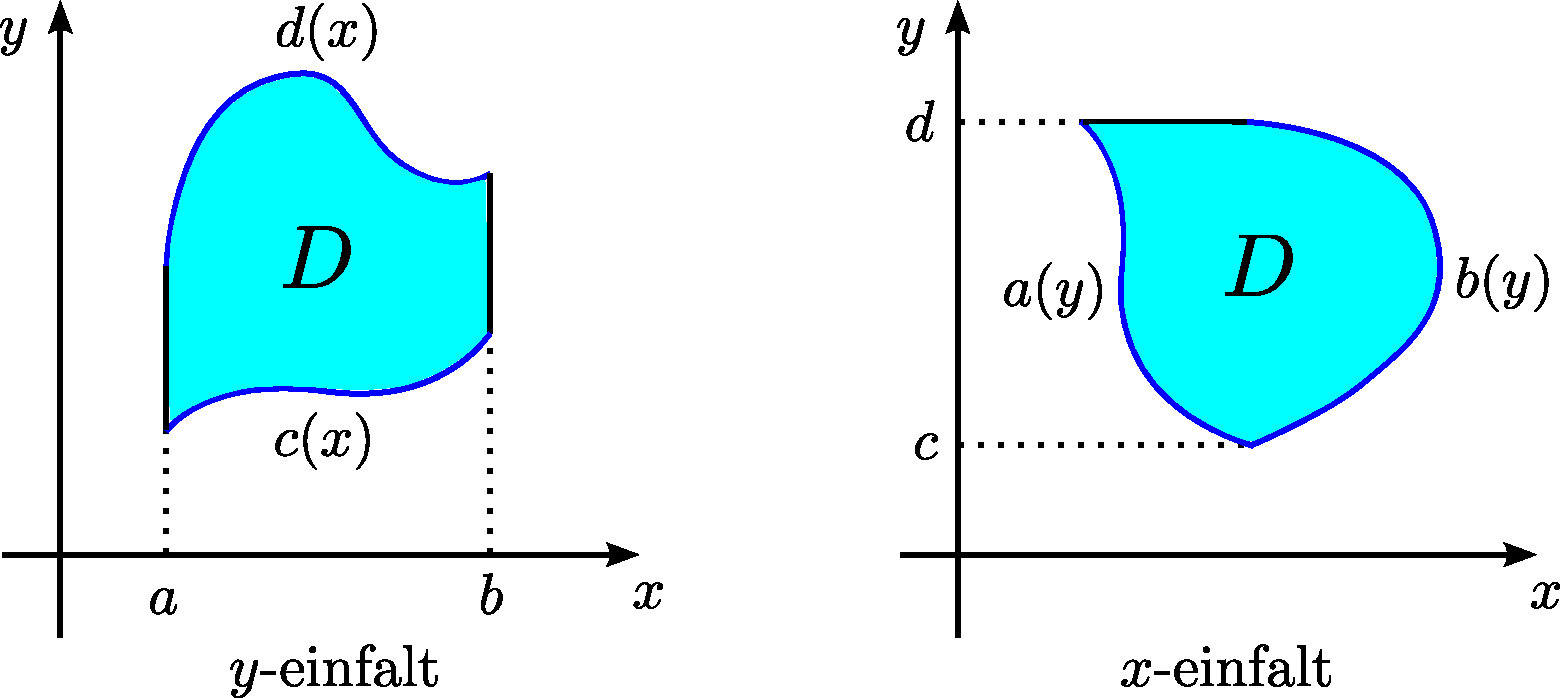
\includegraphics[width=0.65\linewidth]{einfalt}
            \caption*{}
\end {figure}
\end{frame}


\begin{frame}{$x$-einföld og $y$-einföld svæði} 

\begin {block}{Regla \kaflanr.\arabic{mycount}}\stepcounter{mycount}
Lokað og takmarkað svæði $D$ í planinu er $y$-einfalt ef og aðeins ef sérhver lína af gerðinni $x=x_0$ sker $D$ í línustriki.  

\medskip
Lokað og takmarkað svæði $D$ er $x$-einfalt ef og aðeins ef sérhver lína af gerðinni $y=y_0$ sker svæðið í línustriki.
\end{block}

\end{frame}



\begin{frame}{Heildi yfir $x$-einföld og $y$-einföld svæði} 

\begin {block}{Setning \kaflanr.\arabic{mycount}}\stepcounter{mycount}
Látum 
$D=\{(x,y)\mid a\leq x\leq b, c(x)\leq y\leq d(x)\}$
vera $y$-einfalt svæði og $f(x,y)$ fall sem er heildanlegt yfir $D$.  Þá er 
$$\tvint_D f(x,y)\,dA=\int_a^b\!\!\!\int_{c(x)}^{d(x)}f(x,y)\,dy\, dx.$$


\medskip
Látum 
$D=\{(x,y)\mid c\leq y\leq d, a(y)\leq x\leq b(y)\}$
vera $x$-einfalt svæði og $f(x,y)$ fall sem er heildanlegt yfir $D$.  Þá er 
$$\tvint_D f(x,y)\,dA=\int_c^d\!\!\!\int_{a(y)}^{b(y)}f(x,y)\,dx\, dy.$$

\end{block}

\end{frame}

\begin {frame}{Heildi yfir $x$-einföld og $y$-einföld svæði}
 \begin {figure}[h!]
 \centering
            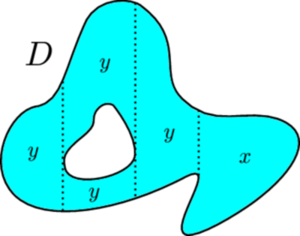
\includegraphics[width=0.35\linewidth]{einfalt2}
            \caption*{Hér er svæðinu $D$ skipt í endanlega mörg $x$-einföld og $y$-einföld svæði sem skarast eingöngu í punktum á jaðrinum.}
\end {figure}
\end {frame}


\begin{frame}{Óeiginleg heildi}
 \begin {block}{Umræða \kaflanr.\arabic{mycount}}\stepcounter{mycount}
  Látum $f(x,y)\geq 0$ vera jákvætt fall sem er skilgreint á svæði $D$ í sléttunni. Ef
  \begin {enumerate}
   \item $D$ er ótakmarkað svæði eða
   \item $f(x,y)$ er ótakmarkað á $D$
  \end {enumerate}
má í sumum tilfellum skilgreina tvöfalda heildið af $f$ yfir $D$.

\medskip
Það er gert með því að finna fyrst runu af stækkandi lokuðum og takmörkuðum mengjum $D_1 \subseteq D_2 \subseteq \cdots \subseteq D$ sem 'stefnir á' $D$. Ef
\begin {equation*}
\tvint_{D_n} f(x,y)\,dA
\end {equation*}
er vel skilgreint fyrir öll $n$ og hefur markgildi þegar $n\to \infty$ (fyrir allar ólíkar runur $(D_n)_{n\geq 1}$) þá 
skilgreinum við \emph{óeiginlega heildið}
\begin {equation*}
 \tvint_{D} f(x,y)\,dA := \lim_{n\to \infty} \tvint_{D_n} f(x,y)\,dA .
\end {equation*}

\end {block}

\end{frame}




\begin{frame}{} 

\begin {block}{Skilgreining \kaflanr.\arabic{mycount}}\stepcounter{mycount}
 Látum $f$ vera fall sem er heildanlegt yfir svæði $D$ í $\R^2$.  {\em Meðalgildi} fallsins $f$ á $D$ er skilgreint sem talan 
$$\bar{f}=\frac{1}{\mbox{flatarmál }D}\tvint_D f(x,y)\,dA.$$ 
\end{block}

\end{frame}



\begin{frame}{} 

\begin {block}{Skilgreining \kaflanr.\arabic{mycount}}\stepcounter{mycount}
Svæði $D$ í $\R^2$ er sagt vera {\em
  samanhangandi} (e.~connected) ef um sérhverja tvo punkta $P_1$ og $P_2$ í $D$
gildir að til er ferill sem liggur í $D$, byrjar í $P_1$ og endar í
$P_2$.  (Hugtakið sem hér er skilgreint væri venjulega kallað {\em
  ferilsamanhangandi}.) 
\end{block}

\end{frame}



\begin{frame}{} 

\begin {block}{Skilgreining \kaflanr.\arabic{mycount}}\stepcounter{mycount}
(Meðalgildissetning fyrir tvöföld heildi)
Gerum ráð fyrir að $f$ sé samfellt fall sem er skilgreint á lokuðu, takmörkuð og samanhangandi svæði $D$ í $\R^2$.   Þá er til punktur $(x_0,y_0)$ í $D$ þannig að 
$$\frac{1}{\mbox{flatarmál }D}\tvint_D f(x,y)\,dA=f(x_0,y_0).$$
\end{block}

\end{frame}

\end{document}